% ----------------------------------------------------------
\chapter{REFERENCIAL TEÓRICO}\label{cap:desenvolvimento}
% ----------------------------------------------------------
\subsection{Contratação de serviços gerais}

A contratação de serviços é uma prática fundamental para o funcionamento de empresas e organizações em diferentes setores da economia. Ao longo das últimas décadas, o processo de contratação de serviços passou por transformações significativas devido ao avanço da tecnologia, mudanças nas práticas de negócios e a evolução das necessidades e expectativas dos clientes.
No final do século 20, conforme observado por \textcite{TheHiringProcess1994} a contratação de serviços era caracterizada por processos mais tradicionais e burocráticos. As empresas geralmente buscavam serviços através de licitações, onde eram estabelecidos requisitos e critérios para seleção de fornecedores. Os documentos físicos, como propostas e contratos, eram trocados por correio ou entregues pessoalmente. A comunicação entre as partes envolvidas era principalmente feita por telefone ou reuniões presenciais. As informações sobre os fornecedores eram obtidas por meio de referências, contatos pessoais e catálogos impressos. Esse processo era muitas vezes demorado e limitado em termos de alcance e acesso a informações.
Atualmente, a contratação de serviços passou por uma transformação significativa, impulsionada pela digitalização e pela crescente interconectividade. A internet e as tecnologias digitais desempenharam um papel fundamental na simplificação e agilização desse processo. Agora, as empresas podem acessar uma ampla variedade de serviços por meio de plataformas online especializadas, marketplaces e diretórios digitais. A contratação de serviços também se tornou mais transparente, permitindo uma comparação mais fácil entre diferentes fornecedores.

% \subsection{Contratação de Serviços Gerais antigamente}
% A presença de um aplicativo móvel pode variar de acordo com o setor, tamanho da empresa e modelo de negócio. 
% Algumas empresas podem optar por não desenvolver um aplicativo móvel se considerarem que sua prestação de serviços pode ser melhor realizada por meio de outros canais de comunicação.

% Alguns exemplos de empresas de prestação de serviços que geralmente não possuem aplicativos dedicados:
% \begin{itemize}[label=$\bullet$]
% 	\item Empresas de consultoria: Consultorias em gestão, finanças, recursos humanos e outras áreas costumam oferecer serviços sem a necessidade de um aplicativo. A comunicação e interação com os clientes são realizadas principalmente por meio de reuniões presenciais, chamadas telefônicas, e-mails e outras formas de comunicação convencionais.
% 	\item Empresas de construção: Empresas de construção, como empreiteiras e empresas de arquitetura, geralmente não dependem de aplicativos para a prestação de serviços. A comunicação com os clientes é feita pessoalmente, por telefone ou por e-mail, e o trabalho é coordenado de forma tradicional no local de construção.
% 	\item Prestadores de serviços locais: Muitos prestadores de serviços locais, como encanadores, eletricistas, jardineiros, serviços de limpeza, entre outros, fornecem serviços sem a necessidade de um aplicativo. A comunicação e agendamento de serviços são realizados diretamente com os clientes por telefone, e-mail ou pessoalmente.
% \end{itemize}
% Essas empresas geralmente dependem de comunicação direta com os clientes por meio de reuniões presenciais, telefonemas, e-mails, plataformas online de compartilhamento de documentos e outros meios de comunicação eletrônica.

% \subsection{ Como a contratação tem sido realizada ao longo dos anos}
% As contratações de prestação de serviços têm evoluído de várias maneiras. Algumas tendências e mudanças que têm sido observadas:
% \begin{itemize}[label=$\bullet$]
% 	\item Digitalização: Com o avanço da tecnologia, o processo de contratação de serviços tem se tornado cada vez mais digital. Plataformas online e sites especializados têm surgido, conectando clientes e prestadores de serviços de forma mais rápida e eficiente. Isso inclui sites de freelancers, marketplaces e aplicativos móveis.
% \end{itemize}
% A contratação de serviços costumava ocorrer de maneira mais tradicional e localizada.

% \begin{itemize}[label=$\bullet$]
% 	\item Indicação boca a boca: As recomendações de amigos, familiares e conhecidos desempenhavam um papel importante na contratação de serviços. As pessoas confiavam em indicações diretas de pessoas de confiança para encontrar prestadores de serviços.
% 	\item Anúncios impressos e diretórios: Os anúncios em jornais, revistas, panfletos e diretórios impressos eram comuns. As empresas de serviços pagavam por espaços publicitários nessas mídias para se promoverem.
% 	\item Consulta em pessoa ou por telefone: Os clientes entravam em contato com os prestadores de serviços por telefone ou visitavam pessoalmente suas lojas, escritórios ou estabelecimentos para obter informações, fazer perguntas e agendar serviços.
% 	\item Papelada física: Os contratos, acordos e documentos relacionados eram geralmente preenchidos e assinados em papel físico. Isso exigia a troca de documentos em mãos ou por correio.
% \end{itemize}
% É importante ressaltar que, embora essas práticas tradicionais ainda existam em algumas áreas e localidades, a tecnologia e a digitalização transformaram significativamente a maneira como a contratação de serviços é realizada atualmente, proporcionando maior conveniência, alcance global e acesso a informações relevantes.

\subsection{Comparação}
\subsubsection{GetNinjas}
No momento, a GetNinjas é a plataforma com maior destaque, pois possui uma grande variedade de profissionais de diversas áreas diferentes.
O aplicativo está disponível tanto para Android quanto para iOS. O sistema é dividido em dois aplicativos, um para o cliente e outro para o
prestador de serviços. A forma de negociação entre o cliente e o prestador acontece fora da plataforma, onde o prestador deve entrar em contato com as informações disponibilizadas pelo cliente. No entanto, esse modelo pode estar gerando alguns gargalos, pois dificulta a comunicação entre as partes. Vale ressaltar que a plataforma não gerencia o processo de pagamento entre o cliente e o prestador. Na verdade, o prestador compra "moedas" no aplicativo e, com essas "moedas", ele pode ter acesso aos contatos de quem está anunciando.
\subsubsection{99freelas}
A 99freelas é uma plataforma estabelecida e reconhecida que atende principalmente profissionais da área de tecnologia, embora também abranja
outras áreas. Ela oferece uma maneira conveniente para os freelancers encontrarem projetos adequados às suas habilidades e interesses.
Como intermediadora entre o prestador de serviço e o cliente, a 99freelas desempenha um papel importante na facilitação das transações.
Uma das principais vantagens da plataforma é a gestão dos pagamentos, o que proporciona confiabilidade tanto para o prestador de serviço 
quanto para o cliente. A 99freelas geralmente cuida da forma de pagamento, garantindo que o profissional seja remunerado adequadamente e 
que o cliente tenha segurança na transação financeira.

\begin{table}[htb]
    \centering
    \caption{Comparação}
    \label{tab:comparação}
\begin{tabular}{|p{5cm}|p{2cm}|p{2cm}|p{2cm}|}
    \hline
    \textbf{Características} & \textbf{GetNinjas} & \textbf{99freelas} & \textbf{Empregai}  \\ \hline
    Diversidade de serviços   & \multicolumn{1}{c|}{\textbf{X}}   & \multicolumn{1}{c|}{\textbf{-}}  & \multicolumn{1}{c|}{\textbf{X}} \\ \hline
	Avaliações e recomendações   & \multicolumn{1}{c|}{\textbf{X}}   & \multicolumn{1}{c|}{\textbf{X}}  & \multicolumn{1}{c|}{\textbf{X}} \\ \hline
    Aplicativo móvel   & \multicolumn{1}{c|}{\textbf{X}}   & \multicolumn{1}{c|}{\textbf{-}}  & \multicolumn{1}{c|}{\textbf{X}} \\ \hline
    Sistema de mensagens   & \multicolumn{1}{c|}{\textbf{?}}   & \multicolumn{1}{c|}{\textbf{X}}  & \multicolumn{1}{c|}{\textbf{X }} \\ \hline
    Possibilidade dos clientes se adicionar   & \multicolumn{1}{c|}{\textbf{-}}   & \multicolumn{1}{c|}{\textbf{-}}  & \multicolumn{1}{c|}{\textbf{X}} \\ \hline
	Avaliação de pessoas conhecidas   & \multicolumn{1}{c|}{\textbf{-}}   & \multicolumn{1}{c|}{\textbf{-}}  & \multicolumn{1}{c|}{\textbf{X}} \\ \hline
	Pagamentos na plataforma   & \multicolumn{1}{c|}{\textbf{-}}   & \multicolumn{1}{c|}{\textbf{X}}  & \multicolumn{1}{c|}{\textbf{X}} \\ \hline
\end{tabular}
    \fonte{Elaborado pelos autores (2023).}
\end{table}

% ----------------------------------------------------------
\subsection{Modelo incremental}

% ----------------------------------------------------------
De acordo com \textcite{Pressman2016} os modelos tradicionais de processos de desenvolvimento se concentram em estruturar e ordenar o desenvolvimento de software. 
Nesses modelos, as atividades e tarefas ocorrem sequencialmente, seguindo diretrizes de progresso bem definidas. O autor também define algumas atividades genéricas
para os processos de desenvolvimento de software, que são:
\begin{itemize}[label=$\bullet$]
	\item Comunicação: Levantamento de requisitos.
	\item Planejamento: Estimativas, cronograma, acompanhamento.
	\item Modelagem: Análise, projeto.
	\item Construção: Código, testes.
	\item Entrega/Disponibilização: Entrega, feedback.
	\end{itemize}
	De acordo com \textcite{Pressman2016}, o modelo incremental combina os fluxos de processo linear e paralelo dos elementos. Esse modelo é aplicado por
	meio de sequências lineares escalonadas à medida que o tempo avança. Cada sequência linear produz incrementos entregáveis do software.
	\textcite{Pressman2016} destaca que, ao utilizar um modelo incremental, o primeiro incremento frequentemente é um produto essencial, fundamental 
	para atender às necessidades iniciais do cliente. Esse produto essencial é utilizado pelo cliente ou passa por uma avaliação detalhada para obter feedback valioso. 
	Com base no uso e/ou na avaliação, é desenvolvido um planejamento para o próximo incremento, levando em consideração as modificações necessárias para melhor adequar o 
	produto às necessidades do cliente, bem como a entrega de recursos e funcionalidades adicionais.
	\newline Dessa forma, o projeto em questão tem como objetivo utilizar o processo incremental para o desenvolvimento do software Empregai, seguindo validações de progresso quinzenais.

\subsection{React Native}
O React Native é uma poderosa ferramenta de desenvolvimento que permite criar aplicativos móveis nativos para iOS e Android usando JavaScript e a biblioteca React. Essa abordagem eficiente e produtiva para a criação de aplicativos móveis multiplataforma tem impulsionado o crescimento do React Native no mercado.

Desenvolvido e mantido pela empresa META, também proprietária do Facebook, o framework React Native é altamente confiável, beneficiando-se de uma comunidade ativa 
que disponibiliza uma ampla gama de conteúdos gratuitos online. A tendência atual para novos aplicativos móveis é o desenvolvimento voltado principalmente para as 
plataformas Android e iOS. Com o React Native, é possível adotar uma abordagem híbrida, permitindo a construção simultânea de um produto para ambas as plataformas, 
evitando a necessidade de desenvolvimento separado usando as linguagens nativas de cada plataforma, conforme destacado por (\textcite{Sabino}).

Outro fator determinante na escolha do React Native como framework é a sua curva de aprendizado acessível. Devido à ampla familiaridade e popularidade da linguagem 
JavaScript no mundo do desenvolvimento, a adoção do React Native é evidente (Figura 1), destacando sua força e importância no mercado.
\begin{figure}[htb]
	\caption{\label{fig:Fig_1}Linguagens mais utilizadas Fonte: \cite{Softermii}}
	\begin{center}
		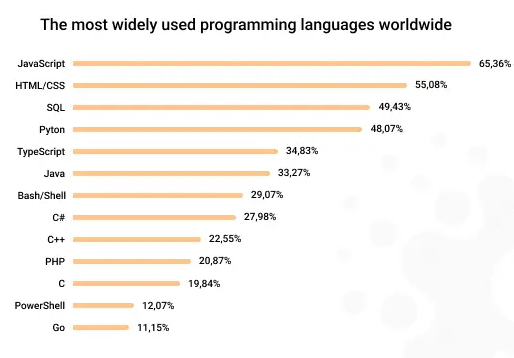
\includegraphics{images/top.png}
	\end{center}
\end{figure}
% ----------------------------------------------------------

\subsection{Expo}
O Expo é uma plataforma que simplifica o desenvolvimento de aplicativos móveis usando JavaScript e React Native. Com recursos nativos do dispositivo acessíveis e facilitando a colaboração e distribuição de aplicativos, o Expo oferece uma solução abrangente para criar aplicativos móveis.

Segundo (\textcite{Hugo}) o uso do Expo proporciona uma camada de abstração superior ao React Native, resultando em uma experiência aprimorada no desenvolvimento de software. Com o aumento do 
número de usuários de smartphones, especialmente nas plataformas Android e iOS, a necessidade de criar aplicativos para ambas as plataformas se tornou cada vez mais 
evidente. Nesse contexto, o Expo oferece uma vantagem no desenvolvimento híbrido, simplificando o processo de criação de aplicativos multiplataforma.

\begin{figure}[htb]
	\caption{\label{fig:Fig_1}Expo vantagens Fonte: \cite{Expo}}
	\begin{center}
		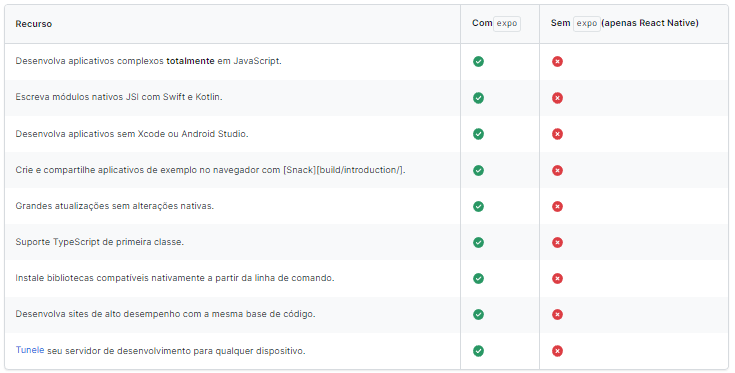
\includegraphics[width=0.8\textwidth]{images/expo.png}
	\end{center}
\end{figure}

\subsection{Gin}
O framework Gin é uma biblioteca leve e rápida para construção de APIs em Go. Ele se baseia nos princípios do roteamento HTTP e fornece recursos poderosos para o desenvolvimento de aplicativos web escaláveis e de alto desempenho.

Ao utilizar o Gin, os desenvolvedores se beneficiam de uma sintaxe concisa e intuitiva, o que torna a criação de endpoints mais eficiente e produtiva. O framework oferece um roteamento flexível, permitindo mapear os diferentes endpoints para as funções correspondentes de forma clara e organizada.

Além disso, o Gin oferece suporte para a manipulação de parâmetros nas requisições HTTP. Isso permite que os desenvolvedores acessem e processem os dados enviados pelos clientes de forma simples e segura. O framework também oferece recursos para validação de entrada de dados, facilitando a verificação de formatos, tipos e restrições específicas, garantindo a integridade dos dados recebidos.

Outro aspecto importante do Gin é a sua eficiência e desempenho. Ele foi projetado para ser leve e rápido, proporcionando um processamento ágil das requisições. Isso é especialmente relevante em aplicações de grande escala, onde a capacidade de resposta e o tempo de processamento são cruciais.

O framework Gin também oferece recursos avançados, como middleware, que permite adicionar funcionalidades extras às rotas e endpoints da API. Isso inclui autenticação, autorização, logging e muitos outros aspectos que são essenciais para o desenvolvimento de sistemas seguros e escaláveis.

Em resumo, o uso do framework Gin proporciona uma base sólida e eficiente para o desenvolvimento de APIs RESTful. Sua sintaxe concisa, roteamento flexível, manipulação de parâmetros, validação de entrada e recursos avançados garantem a criação de endpoints robustos, escaláveis e de alto desempenho, possibilitando a construção de aplicações web modernas e eficientes.
